\documentclass[runningheads]{llncs}
\usepackage[T1]{fontenc}
\usepackage{graphicx}
\usepackage{subfiles}
\usepackage[nolist]{acronym}
% \usepackage[backend=biber,style=numeric,]{biblatex}
\usepackage[english=american]{csquotes}
\usepackage{hyperref}
\usepackage{color}
\usepackage{amssymb}
\usepackage[fleqn,tbtags]{mathtools}
\usepackage{minted}
\usepackage{amsmath}
% \usepackage{nccmath}
\usepackage{caption}
\usepackage{algorithm}
\usepackage{wrapfig}
% \usepackage{algpseudocode}
% \usepackage{subcaption}
\usepackage{xcolor} % to access the named colour LightGray
\definecolor{LightGray}{gray}{0.9}

% alter autoref visualization
\def\sectionautorefname{Section}
% subfig setup
\usepackage[labelformat=simple]{subfig}
\renewcommand\thesubfigure{(\alph{subfigure})}
% \renewcommand{\subfigureautorefname}{\figureautorefname}

% \addbibresource{literatur.bib}

\renewcommand*\contentsname{Inhaltsverzeichnis}
\renewcommand*\listfigurename{Abbildungsverzeichnis}
\renewcommand*\listtablename{Tabellenverzeichnis}
\newcommand\algorithmautorefname{Algorithm}
% Content
\newcommand\pLayer{preprocessing layer}
\newcommand\eN{excitatory neuron}
\newcommand\iN{inhibitory neuron}
\newcommand\hMethod{homoeostasis}

\begin{document}

\title{Optimization of Spiking Neural Network}
\author{Klara M. Gutekunst}
\institute{University of Kassel, 34125 Kassel, Germany
\email{klara.gutekunst@student.uni-kassel.com}}

\maketitle
% introduction
\begin{abstract}
The human brain is particularly good at pattern recognition requiring little power. 
Due to this fact, scientists are trying to improve their knowledge of the brain and to build systems to model it.
Since conventional \acfi{ANN} often use backpropagation and are thus, biologically implausible or require a lot of power to do computations researchers have started focusing on implementing alternatives such as \acfi{SNN}.

A \ac{SNN}'s neuron fires if its membrane potential exceeds a certain (adaptable) threshold. 
The membrane's potential is calculated by the sum of incoming spikes with respect their timing.
To make this process more biologically plausible, the membrane potential decays exponentially.
Synapses are modelled by the connections between neurons.
The influence of a synapse on the postsynaptic neuron is represented by the weight of the connection.
This weight is altered during training to disconnect neurons from those that have little influence on their spiking activity.
The usage of \hMethod{} (i.e. adaptive membrane threshold and limiting the firing rate of neurons) prevents single neurons from firing all the time and enables the neurons to learn to different input patterns.

The approach of this paper is tested on the MNIST dataset.  
TODO

\keywords{unsupervised learning \and \acl{STDP} \and biologically plausible \and lateral inhibition \and adaptive spiking threshold \and \hMethod{}}
\end{abstract}
\section{Introduction}

In order to find methods of computation requiring little power consumption, 
researchers have started creating structures modelled on the neurons of the brain.
\acp{SNN} are allegedly suitable means to tackle this task \cite{SNN}.
They differ from normal \acp{ANN} in terms of their architecture and learning method.
Their inputs are 1-bit spike trains as opposed to 32- or 64-bit messages of \acp{ANN} \cite{SNN}.
The input of \acp{SNN} are streams of events which differs from the singular presentation of \acp{ANN} inputs \cite{ANN_SNN_conversion}.
Moreover, instead of backpropagation used for \acp{ANN}, many \ac{SNN} models have different learning rules to optimise their weight, 
such as \acfi{STDP} with exponential time dependence.
The model presented in the following uses \acfi{LIF} neurons and lateral inhibition \cite{SNN}.
Hence, the approach models the leak of current of real neurons, as well as competition among the neurons.

Applications for this approach include pattern recognition \cite{SNN} and object shape recognition \cite{object_detection_SNN,multi_scale_STDP}.
In both cases, the accuracy is surprisingly high for an unsupervised method.

This paper is structured as followed:
In \autoref{sec:main_part} the tackled problem regarding \acp{SNN}, context-specific terms, the network architecture,
 as well as the approach itself is described.
In \autoref{sec:result} the results of tests regarding performance, optimal parameter choice and other metrics of similar approaches are presented.
Methods to train \acp{SNN}, which differ more than the ones outlined in \autoref{sec:result} are described and compared in \autoref{sec:comparison}.
The paper concludes with an outlook in \autoref{sec:conclusion}.

% main part
\section{Main part}
\label{sec:main_part}
This section outlines problems, topic-specific terms, learning methods and architecture of the approach \ac{SNN}.

\section{Problem}
\label{subsec:problem}

Since \acp{SNN} are not only influenced by the input values but also by the temporal dependencies of these inputs, 
algorithms aiming to optimise their parameters are rare.
Moreover, researchers working with \acp{SNN} focus on biologically plausible methods and 
therefore often refuse to use conventional techniques like gradient descent.
\newcommand\rbModel{Rate-based model}
\newcommand\sbModel{Spike-based model}
\subsection{Terms}
\label{subsec:terms}

In this section, technical terms specific to the domain are defined and briefly discussed.

\subsubsection{Spike trains}
are defined as multiple spikes.
\textcolor{red}{
They are encoded as a 1-bit array, where each entry indicates whether a spike (1) or no spike (0) occurred at a certain point in time.
}

\subsubsection{\rbModel{}}
According to \cite{spike_vs_rate} there are two central beliefs with regard to the question of how the neurons communicate with each other.
The firing rate of a neuron is an abstract measurement of the average number of spikes per unit (e.g. duration, neuron, trial).
The \rbModel{} believes that the firing rate captures most of the information, hence the timing of spikes is meaningless.

\subsubsection{\sbModel{}}
According to the \sbModel{}, the firing rate is not sufficient to describe the neural activity.
The spike timing defines spike trains and individual spikes.
As stated in \cite{spike_vs_rate}, the \rbModel{} assumption is stronger than the one of the \sbModel{}.

\subsubsection{Rate-based learning} uses backpropagation during training, but converts the \ac{ANN} to a \ac{SNN} (i.e. transfers trained weights) afterwards. 
According to \cite{SNN} and \cite{STDP_like} the usage of backpropagation is biologically unrealistic.

\subsection{Network architecture}
\label{subsec:architecture}


The \ac{ANN} has an input layer and a \pLayer{} \cite{SNN}.
The input layer consists of $28 x 28$ neurons, i.e. one for each input pixel.
All the neurons of the input layer are connected to all the neurons of the \pLayer{} (all-to-all).

The \pLayer{} has \eN{}s and \iN{}s.
An 1:1 excitatory to inhibitory neuron ratio is chosen, rather than the biologically plausible 4:1 ratio, 
to reduce computional complexity \cite{SNN}.
While every \eN{} is connected to exactly one \iN{} (one-to-one), every \iN{} is connected to all \eN{}s except the one it is already connected to.
The architecture is depicted in \autoref{fig:architecture_SNN}.
This structure creates lateral inhibition and creates competition among the \eN{}s.

\begin{figure}[htbp]
    \center
    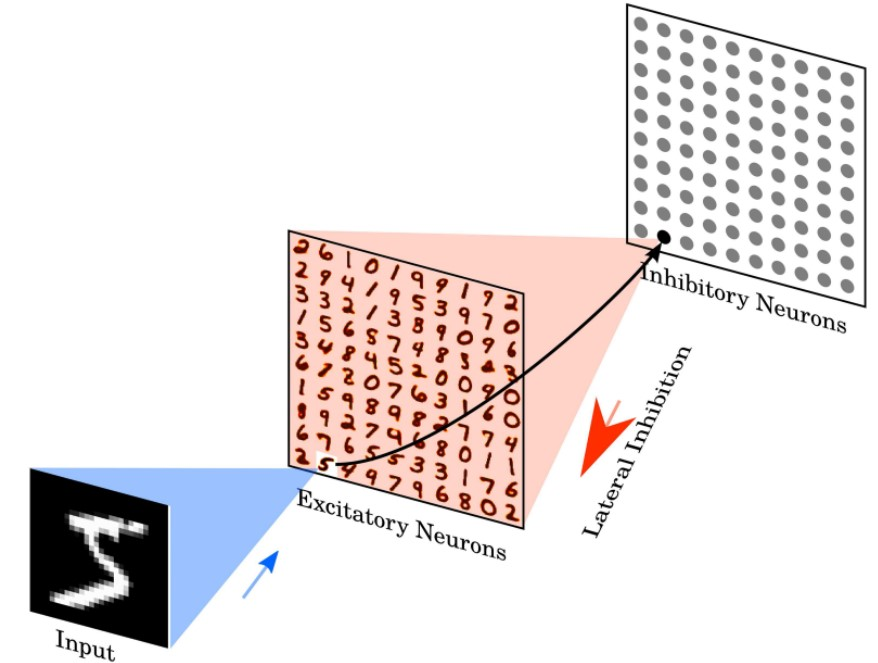
\includegraphics[width=0.5\textwidth]{pictures/architecture_SNN_erste_Quelle.jpg}
    \caption{architecture of the \ac{SNN} from \cite{SNN}}
    \label{fig:architecture_SNN}
\end{figure}
\subsection{Methods}
\label{subsec:methods}

Concepts used in \cite{SNN} include \textcolor{red}{\acfi{LIF} neurons}, \textcolor{red}{lateral inhibition}, \textcolor{red}{synaptic plasticity} and \textcolor{red}{conductance-based synapses}.

\subsubsection{Timing of spikes}
The timing of spikes determines the type of synaptic changes \cite{LTP_D_bio}:
If multiple postsynaptic spikes occur close after presynaptic spikes a \acfi{LTP} is induced, 
whereas repetive postsynaptic spike before the presynaptic ones lead to \acfi{LTD}.


\subsubsection{synaptic plasticity}
Synapses play a crucial role in \ac{SNN} learning tasks such as recognition and computation \cite{Synaptic_plasticity}.
Synaptic plasticity rules is the term used for the different mathematical formulaes realised in activity-dependent modification of synaptic weights.
There is a great variety of synaptic plasticity rules, raging from abstract models to detailed models \cite{Synaptic_plasticity}.

Instances of abstract models include those based on the timing of spikes, such as Pair-based \ac{STDP} models.
\autoref{eq:pair_based_weight_update} from \cite{Synaptic_plasticity} shows the weight update of a pair-based \ac{STDP} model.
$\Delta t = t_{post} - t{pre}$ is the time difference between the presynaptic spike $t_{pre}$ and the postsynaptic spike $t_{post}$.
If a postsynaptic spike arrives with time window $\tau_+$ before a presynaptic one, potentiation occurs, i.e. the synaptic weight is increased. 
Analogously to induce depression the postsynaptic spike needs to precede the presynaptic one within time window $\tau_-$.
The amount of weight change depends on $\Delta t $ and the amplitude parameters $A^+$ and $A^-$.
%
\begin{equation}
    \centering
    \label{eq:pair_based_weight_update}
    \Delta w = \left\{
        \begin{array}{ll}
        \Delta w^+ = A^+ e^{\frac{-\Delta t}{\tau_+}} & \Delta t > 0 \\
        \Delta w^- = -A^- e^{\frac{\Delta t}{\tau_-}} & \Delta t \le 0 \\
        \end{array}
        \right.
\end{equation}
%
Other models, for instance the \ac{TSTDP}, not only take into account a single pair of presynaptic and postsynaptic spikes, 
but triplet combinations of spikes 
(current pre- and post-, current post- and previous post-, current pre- and previous presynaptic one) \cite{Synaptic_plasticity}.

Detailed models on the other hand, may take into account state variables, for instance membrane potential, 
accounting for more biophysically realistic models.
Changes in the synaptic weight of an instance of the \ac{SDSP} model depend on the postsynaptic membrane potential $V_{mem}$ and 
the calcium concentration $C(t)$ \cite{Synaptic_plasticity}.
Whenever a presynaptic spike arrives either potentiation of amount $a$ occurs, if the membrane potential $V_{mem}$ is higher than a certain threshold and the 
calcium concentration $C(t)$ is within certain bounds, or depression of amount $b$ analogously displayed in \autoref{eq:sdsp_weight_update}.
%
\begin{equation}
    \centering
    \label{eq:sdsp_weight_update} 
    W = 
    \left\{
    \begin{array}{ll}
        W + a, \text{if } V_{mem} > V_{mth} \text{ and } \Theta^l_{up} < C(t) < \theta^h_{up}\\
        W - b, \text{if } V_{mem} \le V_{mth} \text{ and } \Theta^l_{dn} < C(t) < \theta^h_{dn}
    \end{array}
    \right.
\end{equation}
%
The \ac{SDSP} approach models synaptic weight $W$ decay as displayed in \autoref{eq:sdsp_weight_decay} from \cite{Synaptic_plasticity}.
If the conditions from \autoref{eq:sdsp_weight_update} are no saisfied or no spike arrives, 
the synaptic weight drifts towards either high or low synaptic weight asymtotes dependent on the weights at a specific time $t$ 
with respect to a threshold $\theta_W$ \cite{Synaptic_plasticity}.
%
\begin{equation}
    \centering
    \label{eq:sdsp_weight_decay}
    \frac{dW(t)}{dt} = 
    \left\{
    \begin{array}{ll}
        \alpha, \text{if } W(t) > \theta_W\\
        - \beta, \text{if } W(t) \le \theta_W\\
    \end{array}
    \right.
\end{equation}
%
Other detailed models, such as \ac{LCP} are outlined in \cite{Synaptic_plasticity}.

\subsubsection{Learning using \ac{STDP}}
The synapses of the \ac{SNN} are trained using unsupervised \acfi{STDP}, which has been observed in a rage of species from insects to humans \cite{STDP_hebbian}. 
The weight of a connection between two neurons models a synapse.
\ac{STDP} is a synaptic learning rule, which adapts weights of synapses according to their degree of causality \cite{STDP_like},
 i.e. how likely the input causes postsynaptic neuron excitation.
\ac{STDP} increases synaptic weight if the postsynaptic neuron reacts immediately after the presynaptic neuron fires \cite{object_detection_SNN}.
The goal of \ac{STDP} is to strengthen synapses of pre- and postsynaptic neuron pairs, 
whose postsynaptic neuron reacts immediately after the presynaptic neuron fires \cite{object_detection_SNN}.
If the postsynaptic neuron fires before the presynaptic one the spike has another origin and thus, the synapse is weakened to disconnect the neurons.
%
\begin{equation}
    \centering
    \label{eq:weight_update}
    \Delta w = \eta (x_{pre} - x_{tar})(w_{max}-w)^\mu
\end{equation}
%
\autoref{eq:weight_update} from \cite{SNN} calculates the weight change after a \textcolor{red}{postsynaptic spike arrives 
(i.e. the synapses' importance is changed according to its influence on the postsynaptic neuron)}.
$\eta$ is the learning rate, presynaptic trace $x_{pre}$ tracks the number of recent presynaptic spikes 
(decaying if no spike arrives, increased by one otherwise), 
$\mu$ is the dependence of the update on the previous weight and 
$x_{tar}$ is the target value of the presynaptic trace at the moment of the postsynaptic spike.
If $x_{tar}$ is high, i.e. many spikes arrived at the postsynaptic neuron, the weight will possibly not be increased 
(especially if fewer spikes arrived at the presynaptic neuron indicated by  $x_{pre}$).

There are also other \ac{STDP} learning rules \cite{SNN}.
Some \ac{STDP} models rely on a teaching signal, which provides the right response \cite{STDP_like}.
Teaching signals are generated by Poison spike generators.
A teaching signal is sent to the correct pool of neurons representing the class (i.e. digit) after a stimulus was presented in the training phase.
The goal of this approach is to make each neuron pool selective to one class of input.


\subsubsection{Competitive Learning}
\textcolor{red}{position schlecht: lateral inhibition und neuron nicht erklärt\\}
The goal of the \ac{SNN}-model is to train its neurons to represent prototypical inputs or an average of similar inputs \cite{SNN}.
To adchieve this goal, the weights of spiking neurons are adapted to become more similar to the input.
Lateral inhibition prevents too many neurons from spiking and thus, prevents them from becoming to similar in the course of adapting to the input.
This results in the receptive fields of the neurons explorating the input space.
To ensure that a approximately constant number of neurons' receptive fields is similiar to an input, 
homoeostasis guarantees similiar firing rates among the neurons.
The learning procedure is similar to k-means-like learning algorithms \cite{SNN}.
Hence, increasing the number of neurons may result in at most 95-97 \% accuracy.


\subsubsection{Neuron model}
\label{subsubsec:neuron_model}
In reality, a neuron fires if the membrane's potential crosses the membrane's threshold $\nu_{thresh}$.
After firing the neuron's membrane potential is reset and within the next few milliseconds cannot spike again \cite{SNN}.
%
\begin{equation}
    \centering
    \label{eq:membrane_vol_pot}
    \tau \frac{dV}{dt} = (E_{rest} - V) + g_e(E_{exc} - V) + g_i(E_{inh} - V)
\end{equation}
%
\autoref{eq:membrane_vol_pot} describes the membrane voltage 
(i.e. the value compared to the threshold $V_{thres}$ which determines whether the neuron fires) change over time constant $\tau$.
$E_{rest}$ is the resting membrane potential, $E_{exc}, E_{inh}$ are equilibrium potentials of excitatory and inhibitory synapses, 
and $g_e, g_i$ the conductances of excitatory and inhibitory synapses (i.e. the influence of respective synapses on membrane voltage of neuron) \cite{SNN}. 
The voltage decays (first parenthesis) and is influenced by the excitatory synapses 
adding to the voltage and the inhibitory synapses subtracting from the voltage.


\subsubsection{Synapse model}
\label{subsubsec:synapse_model}
The synapses' conductance $g_e$/$g_i$ ($e$ excitatory, $i$ inhibitory) model the influence of a presynaptic neuron on another neuron.
If a presynaptic spike arrives at the synapse the weight $w_{i,j}$ between neuron $i$ and neuron $j$ is added to $g_e$/$g_i$.
Otherwise, $g_e$/$g_i$ is decaying.
%
\begin{equation}
    \centering
    \label{eq:exc_conductance}
    \tau_{g_e} \frac{dg_e}{dt} = - g_e
\end{equation}
%
The decay is computed using \autoref{eq:exc_conductance} from \cite{SNN}.
The change over time constant $\tau$ is an \textcolor{red}{exponential decay}.


\subsubsection{\ac{LIF} neurons}
As depicted in \autoref{eq:membrane_vol_pot} from \autoref{subsubsec:neuron_model}, the membrane potential/ voltage $V$'s current leaks out of the neuron 
(i.e. decays without incoming spikes over time).
Due to the exponential decay, these neurons are called \ac{LIF} neurons.


\subsubsection{lateral inhibition}
Since every inhibitory neuron is connected to all excitatory neurons except the one it is already connected to, 
whenever a spike is triggered in an excitatory neuron all inhibitory neurons receive a spike as well.
Hence, neurons that did not fire are inhibited and thus, lateral inhibition and a soft winner-take-all mechanism are created.
An 1:1 excitatory to inhibitory neuron ratio is chosen, rather than the biologically plausible 4:1 ratio, 
to reduce computional complexity \cite{SNN}.





\subsubsection{conductance-based synapses}


\subsubsection{Homoeostasis}
In order to ensure the neurons have a similar firing rate, the \eN{}'s membrane threshold is calculated by $\nu_{thresh} + \theta$, 
where $\theta$ is increased every time the neuron fires and exponentially decaying otherwise.
Since the membrane potential is limited to $E_{exc}$ a neuron stops firing when its membrane threshold is higher than the membrane potential.

This technique countersteers the effect of inhomogeneity of the input and the lateral inhibition.


\subsubsection{Input encoding}
\acp{SNN} transmit information through spikes and thus, analog values have to be encoded into spikes \cite{DIET_SNN}.
There are different types of encodings based on certain beliefs, 
for instance those outlined in \autoref{subsubsec:communication}.
There is a method to encode analog values into spikes \cite{SNN}:
$60,000$ training examples, $10,000$ test examples of $28x28$ pixel images of the digits 0 to 9 compose the MNIST dataset used in \cite{SNN}.
Inputs are Poison spike trains, which are presented for 350ms.
The intensity of a pixel (0 to 255) is proportional to the firing rates (0 to $65.75 Hz$) of the neurons.
If the network does not react to the input, the maximum input firing rate is augmented until it fires in the desired fashion. 


\subsubsection{Training}
In order to allow all variables to decay there is 150ms phase without any input between images.

\subsubsection{Testing}
First the learning rate $\eta$ is set to zero to appoint the neuron's threshold.
After that the training set is presented once more.
The highest response among the ten digit classes is used to assign a class to each neuron, i.e. labels are used.
The predicted value for an input is the class whose neurons have the highest average firing rate.
The classification accuracy is determined on the MNIST test set.

% end section
\section{Results}
\label{sec:result}
% STDP-like paper
The model was evaluated on the MNIST dataset.
According to the authors of \cite{STDP_like}, the dataset is a suitable Benchmark for the \ac{SNN} model, 
since it provides different difficulty levels of categorization.
The authors of \cite{STDP_like} emphasise that the MNIST dataset less complex than biological vision.

The addition to accuracy with regard to the classification of the MNIST dataset impulses \cite{STDP_like} presents \ac{RT} distributions.
\ac{RT} is defined as the time between the presentation of a stimulus and the response (i.e. the first pool to reach the descision pool).
Usually, the \ac{RT} of misclassified digits is higher than the \ac{RT} of correctly classified digits.
However, the network also makes fast errors.
The results were verified with the Kolmogorov-Smirnov test, 
indicating that the correctly and misclassified \ac{RT} distributions are significantly different, 
whereas as the distributions for stimuli from the training and test set were not.

The authors of \cite{STDP_like} compare the performance of the \ac{SNN} model for different training set sizes $n_{train}$.
They find that the network is able to generalize well if the training set size is sufficiently large.
The optimum training set size $n_{train} = 1000$ produced not remarkably higher misclassifaction rates than bigger training set sizes.
The most frequent misclassification was the digit nine as a zero.


% Original STDP paper
In \cite{SNN} the authors compare the performance of the \ac{SNN} model consisting of different numbers of excitatory neurons and different learning rules.
The visualizations suggest that highest number of excitatory neurons (i.e. 6400) produces the best results for all learning rules.
The authors also study propose possible reasons for the distribution of misclassified digits.
The most common misclassification was the digit four as a nine.

The authors of \cite{SNN} include a table visualizing performances of different \acp{SNN}.
Rate-based learning methods adchieve the best results.


Benchmark\\
zugrundeliegende Daten
\section{Comparison}
\label{sec:comparison}

% STDP-like paper
The \ac{SNN} model from \cite{STDP_like} determines its output by 
choosing the class of the first neuron pool to reach the descision threshold with its accumulated sensory evidence.
The authors claim that the original method of using a majority vote of single threshold-based neuron acticity is less biologically plausible.


to other implementations

to biology


\section{Evaluation}
\label{sec:evaluation}

\subsubsection{Inhibition}

\subsubsection{Spike-based Learning in ML}

\subsubsection{Competitive Learning}

\subsubsection{Robustness} 
\section{Conclusion and Outlook}
wdhl wie gut es ist\\
was kommt noch?\\
wie zu verbessern?

\begin{acronym}[XXXX]
    \acro{SNN}[SNN]{spiking neural network}
    \acro{ANN}[ANN]{artificial neural network}
    \acro{STDP}[STDP]{spike-timing-dependent plasticity}
    \acro{LIF}[LIF]{leaky-integrate-and-fire}
    \acro{SVM}[SVM]{support vector machines}
    \acro{kNN}[kNN]{k-means clustering}
    \acro{NN}[NN]{neural networks}
    \acro{CNN}[CNN]{convolutional neural networks}
    \acro{LSTM}[LSTM]{long short-term memory networks}
    \acro{SOM}[SOM]{self-organized map}
\end{acronym}

%\bibliographystyle{alphadin}
\bibliographystyle{splncs04}
\bibliography{literatur}

% \printbibliography
\end{document}